\chapter{Methodology}
\label{ch:methodology}

This chapter documents how the system was built: how the dataset and its labels
were constructed, how the feature set was selected and the cascade trained, how
the guideline knowledge base was assembled and indexed, how the prompts were
engineered, how the fine-tuning corpus was generated, and how the safety
validator was implemented.

\section{Dataset}
\label{sec:dataset}

\subsection{Source}

The screening model is trained on the National Health and Nutrition Examination
Survey (NHANES) 2021--2023 cycle, published by the Centers for Disease Control
and Prevention and the National Center for Health Statistics
\cite{nhanes2021}. NHANES combines an in-home interview with a standardised
physical examination and laboratory panel administered in a mobile examination
centre, and is designed to be representative of the non-institutionalised
civilian population of the United States. It was selected for three reasons:
it is the most recent publicly available cycle; it contains, in a single
linked record per participant, both the routine measurements used as model
inputs and the kidney markers required to construct the label; and it is a
cross-sectional survey of an unselected population, so the class prior it
exhibits is representative of a screening setting rather than of a nephrology
clinic.

Adult participants with the required measurements available were retained,
yielding a modelling cohort of 5{,}552 participants. Data preparation was
performed in a leakage-aware manner: the extraction, cleaning and splitting
were completed before any modelling, and the resulting file was
hash-verified at training time to guarantee that the audited dataset and the
trained artefact correspond.

\subsection{Target label construction}

The target variable is a three-level screening category derived from the KDIGO
risk grid \cite{kdigo2024} using the participant's measured \eGFR{} and \UACR,
as shown in Figure~\ref{fig:kdigo}. The KDIGO ``very high'' cell group is merged
into the \textbf{high} category, since the operational consequence for a
screening tool---urgent referral for confirmatory assessment---is identical.

\begin{figure}[H]
\centering
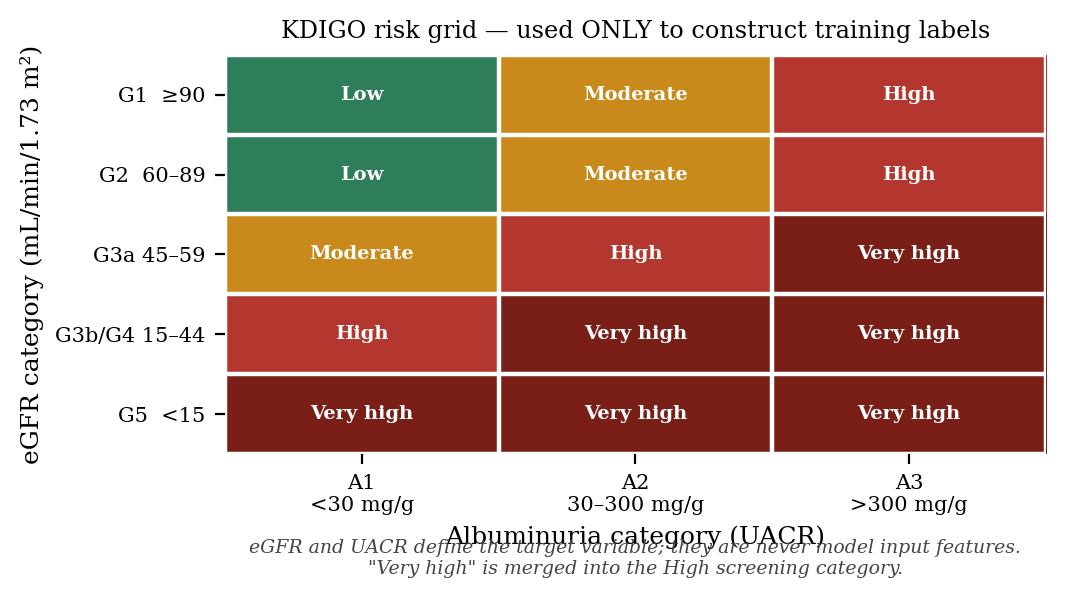
\includegraphics[width=0.72\textwidth]{fig_kdigo_grid.png}
\caption{The KDIGO risk grid used to construct the target label. Both axes are
laboratory kidney markers; they define what the model predicts and are never
supplied to it as inputs.}
\label{fig:kdigo}
\end{figure}

This is the pivotal methodological decision of the ML component and merits
emphasis. The markers \eGFR{} and \UACR{} appear \emph{only} on the label side
of the learning problem. They are removed from the feature matrix before any
model sees the data. The learning task is therefore: predict a
laboratory-defined kidney-risk stratification using only measurements that do
not include the defining laboratory tests.

\subsection{Splits and class distribution}

The cohort was partitioned into a training set, a validation set used for model
selection and threshold tuning, and a test set held out entirely from
development. The union of training and validation constitutes the
\emph{development} set on which the deployed model is finally refitted.
Table~\ref{tab:splits} and Figure~\ref{fig:classdist} give the resulting sizes
and class composition.

\begin{table}[H]
\centering
\caption{Dataset splits and class distribution (NHANES 2021--2023).}
\label{tab:splits}
\begin{tabular}{@{}lrrrr@{}}
\toprule
\textbf{Split} & \textbf{N} & \textbf{Low} & \textbf{Moderate} & \textbf{High} \\
\midrule
Train & 3{,}886 & 3{,}222 & 491 & 173 \\
Validation & 833 & 691 & 105 & 37 \\
\midrule
Development (deployed fit) & 4{,}719 & 3{,}913 & 596 & 210 \\
Test (held out) & 833 & 690 & 105 & 38 \\
\bottomrule
\end{tabular}
\end{table}

\begin{figure}[H]
\centering
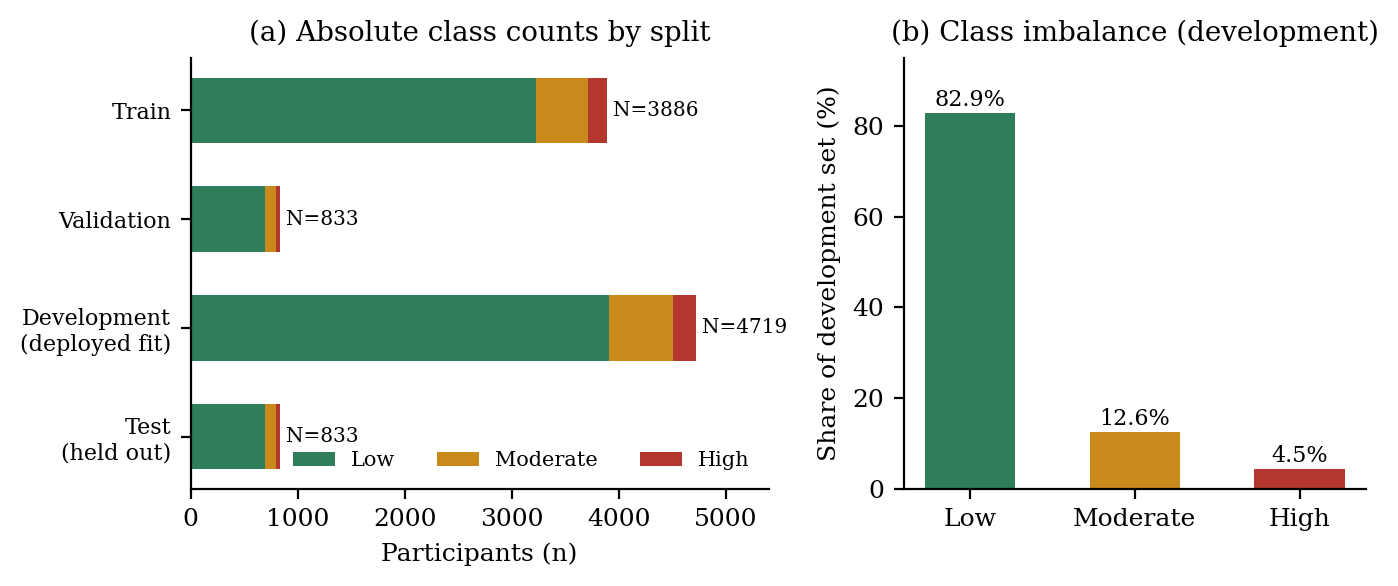
\includegraphics[width=\textwidth]{fig_class_distribution.png}
\caption{Class distribution across splits. The high-risk class represents only
4.5\% of the development set, which dominates the modelling strategy.}
\label{fig:classdist}
\end{figure}

The imbalance is severe: 82.9\% low, 12.6\% moderate and 4.5\% high in the
development set. A trivial classifier predicting ``low'' for every participant
would achieve 82.9\% accuracy while detecting nobody, which is why aggregate
accuracy is not used as the primary criterion anywhere in this work.

\section{Feature Set}
\label{sec:features}

\subsection{Selection}

An initial pool of 22 candidate variables was assembled from the routinely
measured NHANES items. Feature selection during model development---driven by
cross-validated contribution to each stage---reduced this to fourteen unique
model inputs. The variables that did not survive selection into either stage
were sex, body mass index, resting pulse, serum sodium, serum potassium,
borderline-diabetes status, high-cholesterol history and cholesterol-medication
use.

The two stages consume overlapping but distinct subsets: Stage~1 uses thirteen
features and Stage~2 uses six, with serum albumin appearing only in Stage~2 and
eight variables appearing only in Stage~1. Table~\ref{tab:features} lists the
final set.

\begin{table}[H]
\centering
\caption{The fourteen deployed model inputs, with stage membership.
Stage-1 order reflects the selection ranking within that stage.}
\label{tab:features}
\small
\begin{tabular}{@{}llccc@{}}
\toprule
\textbf{Feature} & \textbf{Unit / type} & \textbf{Stage 1} &
\textbf{S1 order} & \textbf{Stage 2} \\
\midrule
\multicolumn{5}{@{}l}{\emph{Demographic and socioeconomic}}\\
age & years & \checkmark & 1 & \checkmark \\
income\_poverty\_ratio & ratio & \checkmark & 10 & \\
\midrule
\multicolumn{5}{@{}l}{\emph{Anthropometric and vital signs}}\\
waist & cm & \checkmark & 13 & \\
mean\_sbp & mmHg & \checkmark & 5 & \checkmark \\
mean\_dbp & mmHg & \checkmark & 11 & \\
\midrule
\multicolumn{5}{@{}l}{\emph{Routine blood chemistry}}\\
glucose & mg/dL & \checkmark & 6 & \\
hba1c & \% & \checkmark & 3 & \\
blood\_urea\_nitrogen & mg/dL & \checkmark & 2 & \checkmark \\
uric\_acid & mg/dL & \checkmark & 8 & \checkmark \\
serum\_albumin & g/dL & & --- & \checkmark \\
hemoglobin & g/dL & \checkmark & 12 & \checkmark \\
\midrule
\multicolumn{5}{@{}l}{\emph{Self-reported comorbidity history (binary)}}\\
diabetes\_yes & 0/1 & \checkmark & 9 & \\
hypertension\_doctor\_told & 0/1 & \checkmark & 7 & \\
taking\_bp\_medicine & 0/1 & \checkmark & 4 & \\
\bottomrule
\end{tabular}
\end{table}

Two observations are worth noting. First, blood urea nitrogen ranks second in
Stage~1 and is retained in Stage~2. BUN is a nitrogenous waste product cleared
by the kidneys, and is part of a standard basic metabolic panel---unlike
creatinine, it is being used here as a routinely available correlate rather
than as the creatinine-based marker that defines the label. Second, the Stage-2
subset is dominated by continuous physiological quantities (BUN, uric acid,
haemoglobin, serum albumin, systolic pressure, age), consistent with its role of
grading severity among individuals already flagged as at risk.

\subsection{Preprocessing and missing values}

Each stage carries its own fitted \texttt{ColumnTransformer}, serialised inside
the model package, which applies median imputation to numeric features and
most-frequent imputation to binary features, with the imputation statistics
learned on the training data only.

One domain-specific consistency rule is applied at inference time before the
feature vector is constructed: if a user reports no diagnosed hypertension and
leaves the blood-pressure-medication field blank, that field is set to $0$
rather than treated as missing. This mirrors the structural-missingness
convention used when the dataset was prepared---a person without a hypertension
diagnosis is not on antihypertensive medication---and prevents a distribution
shift between training and serving.

The count and identity of every imputed field is retained and returned with the
prediction, and feeds directly into the reliability rule of
Equation~\ref{eq:reliability}.

\section{Handling Class Imbalance}
\label{sec:imbalance_method}

Resampling is applied inside the training pipeline of each stage, never to the
validation or test data, so that reported metrics reflect the true class prior.

Stage~1 uses random over-sampling of the minority (at-risk) class to parity
(\texttt{sampling\_strategy} $=1.0$). Stage~2 operates on the smaller at-risk
subpopulation, where the high/moderate ratio is roughly 1:3, and uses a hybrid
over/under-balancing scheme that synthesises minority neighbours
($k=7$) while removing a fraction (0.25) of majority examples, targeting a 1:1
ratio.

\section{Model Development}
\label{sec:model_dev}

\subsection{Algorithms and hyperparameters}

Stage~1 is a random forest \cite{breiman2001} and Stage~2 a gradient-boosting
classifier \cite{friedman2001}. Both are deliberately shallow: the forest is capped at depth 5 and the boosting model at
depth 2, with a low learning rate. Given a minority class of only a few hundred
examples, constraining capacity was found to matter more than adding it.
Table~\ref{tab:hyper} lists the final configuration.

\begin{table}[H]
\centering
\caption{Final model configuration of the deployed cascade.}
\label{tab:hyper}
\small
\begin{tabularx}{\textwidth}{@{}L{1.55in} X@{}}
\toprule
\textbf{Component} & \textbf{Parameters} \\
\midrule
Stage-1 Random Forest & \texttt{n\_estimators}=150, \texttt{max\_depth}=5,
\texttt{max\_features}=sqrt, \texttt{min\_samples\_leaf}=2,
\texttt{min\_samples\_split}=2, \texttt{bootstrap}=true,
\texttt{max\_samples}=1.0 \\
Stage-1 resampler & RandomOverSampler, \texttt{sampling\_strategy}=1.0 \\
Stage-2 Gradient Boosting & \texttt{n\_estimators}=150,
\texttt{learning\_rate}=0.05, \texttt{max\_depth}=2,
\texttt{min\_samples\_leaf}=1, \texttt{min\_samples\_split}=2,
\texttt{subsample}=1.0 \\
Stage-2 resampler & Over/under balancing, \texttt{k\_neighbors}=7,
\texttt{majority\_remove\_frac}=0.25, \texttt{target\_ratio}=1.0 \\
Cascade thresholds & $\tauone = 0.44$, \quad $\tautwo = 0.50$ \\
Libraries & scikit-learn 1.6.1, imbalanced-learn 0.14.1, NumPy 2.0.2 \\
\bottomrule
\end{tabularx}
\end{table}

\subsection{Validation protocol}

Model selection used repeated stratified cross-validation on the training data
with 5 folds and 3 repeats (15 fits per configuration), with a fixed
cross-validation seed and a fixed model seed for reproducibility. Interval
estimates on the held-out set were obtained by bootstrap resampling with 2{,}000
replicates, and stability across evaluation seeds was checked over five seeds
(42, 52, 62, 72, 82). The complete configuration is captured by a fingerprint
recorded with the run, and the deployment package was verified after
serialisation by reloading it and confirming that predictions match the
in-memory model to within $2.2 \times 10^{-16}$.

\subsection{Deployment refit}

Two model instances are distinguished throughout this report. The
\emph{train-only} instance is fitted on the 3{,}886 training records and is used
for development auditing. The \emph{full-development} instance, which is the one
deployed and reported as the final result, is refitted on all 4{,}719
development records (train $+$ validation) with identical hyperparameters and
thresholds, after those hyperparameters and thresholds were frozen. The held-out
test set of 833 participants was never used in either fitting procedure. All
results in Chapter~\ref{ch:results} refer to the deployed full-development
instance unless stated otherwise.

\subsection{Threshold selection}
\label{sec:threshold}

With the classifiers fixed, the two thresholds determine the operating point.
$\tauone$ was selected on development data to prioritise sensitivity of the
at-risk gate, since an individual filtered out at Stage~1 can never be assigned
a non-low category, making a false negative there unrecoverable. The chosen
value of $0.44$ sits below the naive $0.50$, deliberately widening the gate.
$\tautwo$ was left at the neutral $0.50$, as the moderate/high distinction
carries a far smaller asymmetry: both categories generate a referral, differing
only in urgency. Thresholds are stored inside the serialised model package and
read at load time, so re-tuning them does not require a code change.

\section{Explanation Reference Values}
\label{sec:reference}

The perturbation explanation of Equation~\ref{eq:phi} requires a reference value
$r_f$ per feature. These are fixed clinically typical values---age 55 years,
systolic 125 mmHg, diastolic 78 mmHg, glucose 100 mg/dL, HbA1c 5.6\%, BUN
14 mg/dL, uric acid 5.5 mg/dL, serum albumin 4.2 g/dL, haemoglobin 14 g/dL,
waist 98 cm, income-to-poverty ratio 2.0---with all binary comorbidity flags
referenced at $0$ (condition absent). The interpretation of $\phi_f$ is
therefore ``how much does this person's actual value shift the predicted-class
probability, relative to a typical value for that measurement''. These
references are a design choice rather than dataset statistics, and the
explanation is reported as relative to them.

\section{Knowledge Base Construction}
\label{sec:kb}

\subsection{Source selection and scoping}

Ten source documents were collected, spanning professional clinical guidelines
\cite{kdigo2024,kdigo2021bp,adakdigo2022,ada2026,kdoqi2020} and
patient-education material \cite{cdcbasics,cdcprevent,cdcrisk,nkfexercise,syk2015},
listed in Table~\ref{tab:kb}. Each was scoped at
ingestion to the sections relevant to lifestyle, prevention and follow-up;
drug-therapy sections were deliberately excluded from the ingested page ranges,
so that pharmacological content is largely absent from the corpus before any
runtime safety mechanism is applied.

\begin{table}[H]
\centering
\caption{Knowledge-base sources. All are scoped to prevention, lifestyle and
follow-up content.}
\label{tab:kb}
\scriptsize
\begin{tabularx}{\textwidth}{@{}L{1.12in} X L{0.72in} c c@{}}
\toprule
\textbf{ID} & \textbf{Document} & \textbf{Organisation} & \textbf{Year} &
\textbf{Restricted} \\
\midrule
KDIGO2024 & Clinical Practice Guideline for the Evaluation and Management of CKD &
KDIGO & 2024 & \\
KDIGO2021BP & Clinical Practice Guideline for the Management of Blood Pressure in CKD &
KDIGO & 2021 & \\
ADAKDIGO2022 & Diabetes Management in CKD --- ADA/KDIGO Consensus Report &
ADA / KDIGO & 2022 & \\
ADA2026 & Standards of Care in Diabetes, Ch.\ 11: CKD and Risk Management &
ADA & 2026 & \\
KDOQI2020NUTR & KDOQI Clinical Practice Guideline for Nutrition in CKD &
NKF (KDOQI) & 2020 & \checkmark \\
NKFPED & Exercise and Chronic Kidney Disease (patient education) &
NKF & 2026 & \\
CDC\_CKD\_BASICS & Chronic Kidney Disease Basics & CDC & 2024 & \\
CDC\_CKD\_PREVENT & Preventing Chronic Kidney Disease & CDC & 2024 & \\
CDC\_CKD\_RISK & Risk Factors for Chronic Kidney Disease & CDC & 2024 & \\
SYK2015 & Save Your Kidneys --- Complete Guide for Kidney Patients &
Samarpan Kidney Foundation & 2015 & \\
\bottomrule
\end{tabularx}
\end{table}

\subsection{Chunking and annotation}

The scoped sources were segmented into 162 passages of approximately 150 words.
Each passage carries a stable identifier, a topic tag drawn from
\{\texttt{bp}, \texttt{diabetes}, \texttt{nutrition}, \texttt{weight},
\texttt{activity}, \texttt{smoking}, \texttt{sleep}, \texttt{followup},
\texttt{hydration}, \texttt{prevention}, \texttt{general}\}, provenance metadata
(organisation, title, year, URL) used later for citation, and a safety label of
either \texttt{safe\_public} or \texttt{restricted\_clinician\_referral}.

The restriction flag implements the KDOQI constraint \cite{kdoqi2020}. A passage
containing individualised numeric targets for protein, potassium, phosphorus or
sodium is flagged rather than deleted. Flagged passages remain retrievable, but
are rendered into the prompt with an explicit inline marker instructing the
model to refer the reader to a clinician or renal dietitian rather than to
repeat the figure. This preserves the clinical context that makes the advice
coherent while removing the pathway by which a specific number could reach a
patient---and it is backed independently by the validator, which rewrites such
numbers if they appear regardless of their origin.

\section{Retrieval}
\label{sec:retrieval_method}

\subsection{Embedding and indexing}

Passages are embedded with BGE-M3 \cite{chen2024bgem3}, producing 1024-dimensional
dense vectors, and indexed with FAISS \cite{johnson2019faiss}. The embedder is served through a local
Ollama runtime rather than through \texttt{sentence-transformers} directly; the
reason is documented in Chapter~\ref{ch:implementation} and concerns a library
version constraint rather than model quality. The index records the embedder
specification it was built with, and the retriever reconstructs the embedder
from that stored specification at query time, so index-time and query-time
embeddings can never silently diverge.

\subsection{Factor-aware selection}

Query construction and selection follow Algorithm~\ref{alg:retrieval}.

\begin{algorithm}[H]
\caption{Factor-aware retrieval}
\label{alg:retrieval}
\begin{algorithmic}[1]
\Require Attributed factors $\Phi$, risk category $\hat{y}$, knowledge base
$\mathcal{K}$, budget $k$
\Ensure Ordered passage set $\mathcal{R}$, $|\mathcal{R}| \leq k$
\State $q \gets$ risk phrase $\|$ top factor phrases $\|$ mapped clinical terms
  $\|$ intent anchor
\State $T \gets [\,]$
\For{$f \in \Phi$ ordered by $|\phi_f|$, risk-raising factors first}
  \If{$\mathrm{topic}(f)$ defined and $\mathrm{topic}(f) \notin T$}
    \State append $\mathrm{topic}(f)$ to $T$
  \EndIf
\EndFor
\If{$\hat{y} \in \{\text{moderate}, \text{high}\}$ and
    \texttt{followup} $\notin T$}
  \State append \texttt{followup} to $T$
\EndIf
\State $\mathcal{P} \gets \textsc{Search}(\textsc{Embed}(q), \mathcal{K},
  k_{\mathrm{pool}})$ \Comment{score-ordered pool, $k_{\mathrm{pool}} \geq 24$}
\State $\mathcal{R} \gets [\,]$
\For{$t \in T$} \Comment{one best passage per priority topic, in order}
  \If{$|\mathcal{R}| \geq k$} \State \textbf{break} \EndIf
  \State $\kappa \gets$ first unused $\kappa \in \mathcal{P}$ with
    $\mathrm{topic}(\kappa) = t$
  \If{$\kappa$ exists} \State append $\kappa$ to $\mathcal{R}$ \EndIf
\EndFor
\State fill remaining slots of $\mathcal{R}$ from $\mathcal{P}$ by descending score
\State re-sort $\mathcal{R}$ by descending score
\State \Return $\mathcal{R}$
\end{algorithmic}
\end{algorithm}

Figure~\ref{fig:rag} illustrates the process. The essential property is that
line 3--8 make the \emph{selection} depend on the individual, not only the
\emph{ranking}. Without this step, in a corpus this narrow the highest-scoring
passages are near-identical across patients, and per-patient grounding degenerates.

\begin{figure}[H]
\centering
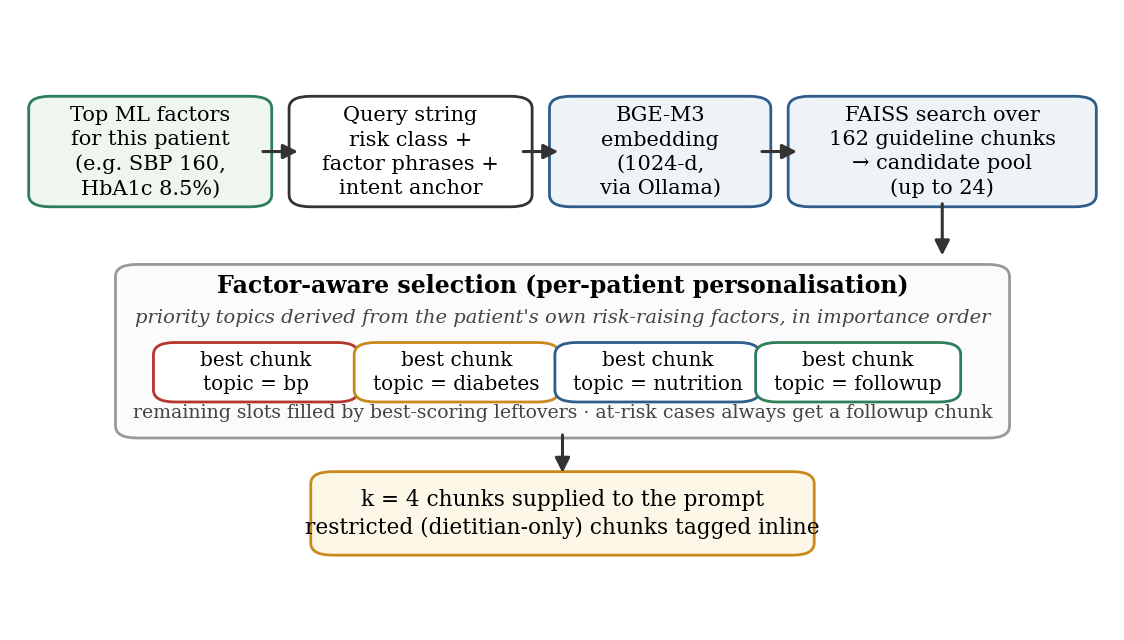
\includegraphics[width=\textwidth]{fig_rag_pipeline.png}
\caption{Factor-aware retrieval. Priority topics are derived from the patient's
own risk-raising factors, guaranteeing per-topic coverage before remaining
slots are filled by similarity.}
\label{fig:rag}
\end{figure}

\section{Prompt Engineering}
\label{sec:prompts}

Two system-prompt variants exist and exactly one is selected automatically per
request, determined by whether a fine-tuned adapter is attached.
Figure~\ref{fig:prompt} shows the anatomy of both turns.

\begin{figure}[H]
\centering
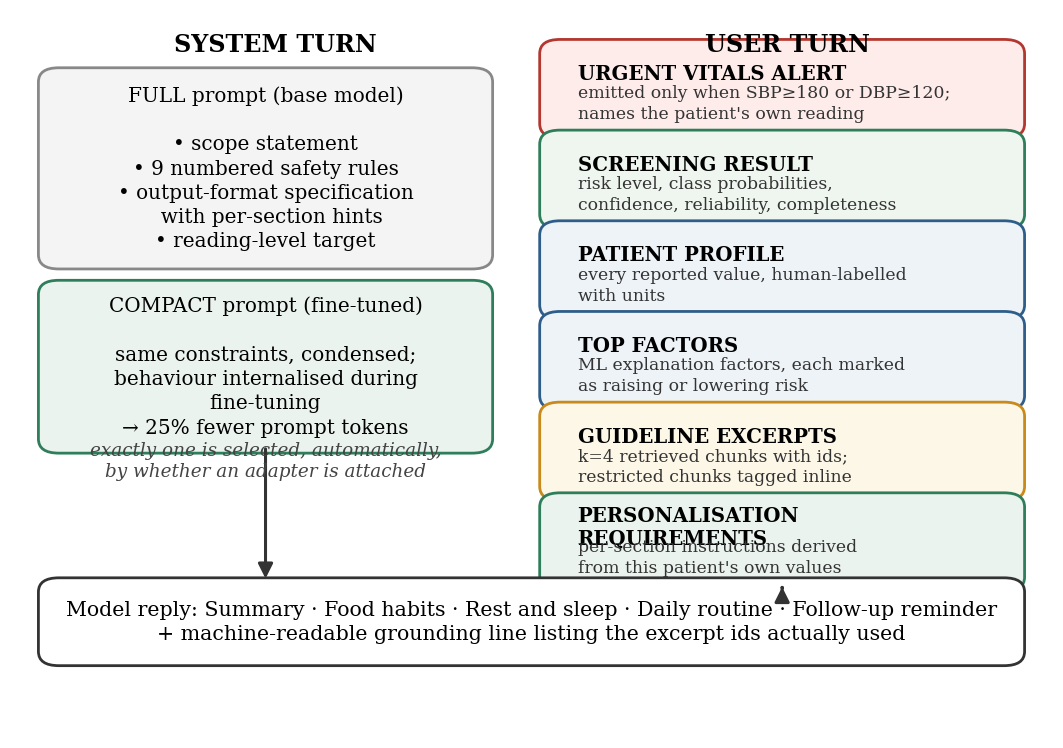
\includegraphics[width=0.95\textwidth]{fig_prompt_structure.png}
\caption{Prompt anatomy. The system turn carries the constraints; the user turn
carries everything patient-specific. The compact variant is selected
automatically when a fine-tuned adapter is active.}
\label{fig:prompt}
\end{figure}

\subsection{The full system prompt}

The full variant states the assistant's scope, enumerates nine safety rules, and
specifies the output format literally. The nine rules are: (1) never state or
imply a diagnosis; (2) never prescribe, recommend, start, stop, change or dose
any medication or supplement; (3) never give individualised numeric targets for
protein, potassium, phosphorus or sodium, deferring instead to a clinician or
renal dietitian; (4) never position the output as a substitute for clinician
judgement, \eGFR{} or \UACR{} testing; (5) \emph{do} tailor wellness education to
the individual's stated conditions; (6) always include a clinician and
laboratory follow-up reminder for a moderate or high result; (7) advise prompt
medical care when the inputs suggest an urgent problem; (8) ground the education
in the supplied guideline excerpts; and (9) write at approximately an
eighth-grade reading level.

Rule 5 deserves comment because it was revised during development. It
originally read ``only give general wellness education'', which the model
followed correctly---producing near-identical generic text for every patient.
The instruction was in direct tension with the personalisation objective. The
revised rule authorises explicit reference to the individual's conditions while
leaving the prohibitions on diagnosis, prescription and numeric targets fully
intact.

\subsection{The compact system prompt}

The compact variant expresses the same constraints and the same output contract
far more briefly, on the premise that a model fine-tuned on full-prompt
behaviour no longer needs the full statement at inference time. This is the
prompt used by the deployed configuration. Its effect on cost is quantified in
Chapter~\ref{ch:results}.

\subsection{The user turn}

The user turn is identical in structure under both variants and contains six
blocks: an urgent-vitals alert (emitted only when systolic $\geq$ 180 or
diastolic $\geq$ 120 mmHg, and naming the individual's own triggering reading);
the screening result with probabilities, confidence and reliability; the
complete patient profile with human-readable labels and units; the attributed
top factors, each marked as raising or lowering risk; the retrieved guideline
excerpts with their identifiers and restriction tags; and a per-section
personalisation requirement block.

The personalisation block is computed in Python from the individual's own values
using transparent threshold rules---for example, elevated blood pressure is
flagged when a hypertension diagnosis is reported or systolic exceeds
130 mmHg---and produces instructions such as ``Food habits: focus on low-sugar,
low-refined-carbohydrate choices because of elevated blood sugar; suggest
reducing salt intake because of high blood pressure''. This block exists because
the abstract instruction to personalise proved insufficient in early testing:
naming the specific fact to reference, and the section to reference it in, was
what actually changed the output.

\section{Training Data Generation}
\label{sec:phase7}

Fine-tuning requires paired examples. Because no corpus of safety-validated,
guideline-grounded kidney education exists, the training corpus was generated by
self-distillation through the system's own pipeline, as shown in
Figure~\ref{fig:datagen}.

\begin{figure}[H]
\centering
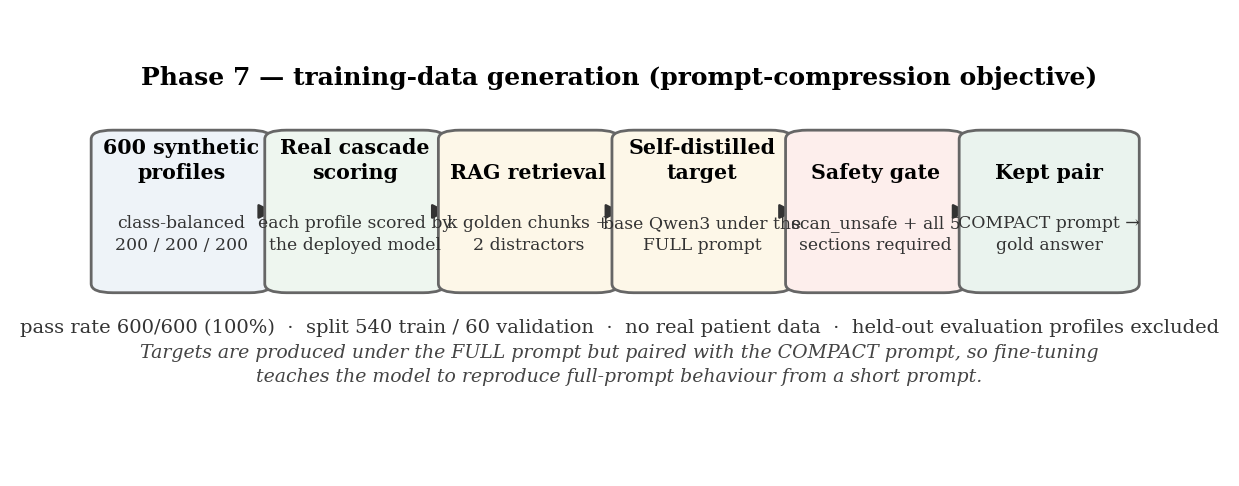
\includegraphics[width=\textwidth]{fig_data_generation.png}
\caption{Training-data generation. Targets are produced under the full prompt
but paired with the compact prompt, making the fine-tuning objective one of
prompt compression.}
\label{fig:datagen}
\end{figure}

Six hundred synthetic patient profiles were generated, balanced at 200 per risk
class. Each profile was scored by the real deployed cascade, so its stated risk
category is the one the production model actually assigns. Retrieval was run for
each profile with four golden passages plus two distractors, and a target answer
was generated by the base Qwen3 model under the \emph{full} prompt. Every
candidate target then had to pass an automated gate: it was rejected unless it
cleared the unsafe-content scan, contained all five required sections, and
mentioned the risk level. All 600 candidates passed, and the corpus was split
540/60 into training and validation.

Two properties of this construction are important. First, the stored example
pairs the \emph{compact} prompt with a target generated under the \emph{full}
prompt, which makes the learning objective explicitly one of prompt
compression---reproducing long-prompt behaviour from a short prompt---rather
than of teaching new clinical content. Second, no real patient data is involved
at any point, and the held-out evaluation profiles and the ML test set were
excluded from the generation pool to prevent leakage into the later evaluation.

\section{Parameter-Efficient Fine-Tuning}
\label{sec:phase8}

The base model is Qwen3-4B-Instruct-2507 \cite{qwen2025}. The adapter was
trained with QLoRA \cite{dettmers2023qlora,hu2022lora}: the base
model's weights were frozen and held in 4-bit NormalFloat quantisation, while
low-rank adapters were trained in bfloat16 on the seven projection matrices of
each transformer block. The relationship between the training-time and
serving-time configurations is shown in Figure~\ref{fig:lora}.

\begin{figure}[H]
\centering
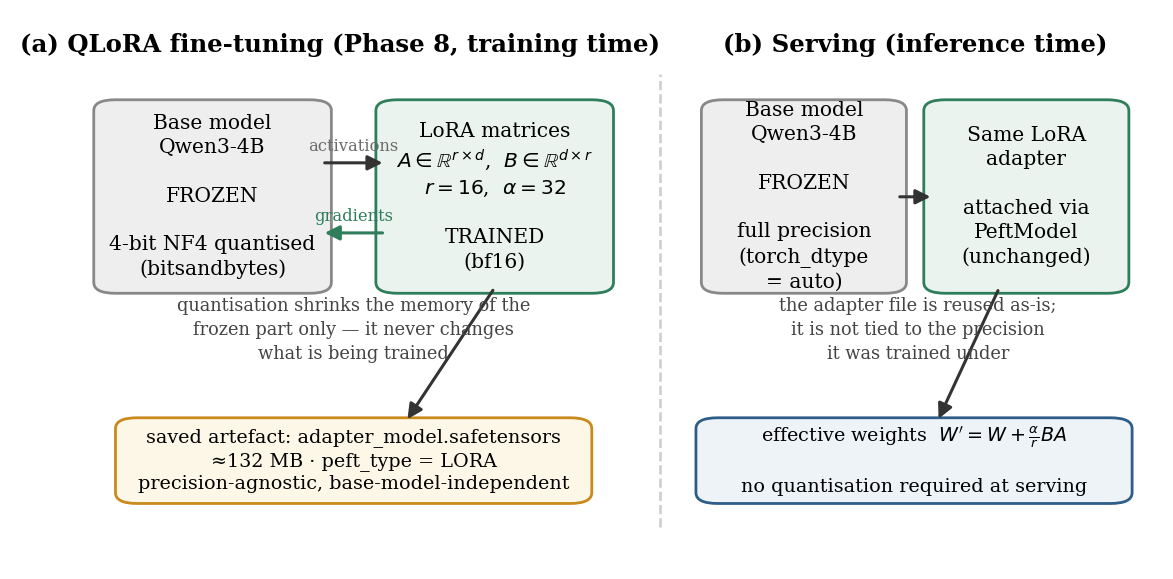
\includegraphics[width=\textwidth]{fig_lora.png}
\caption{QLoRA fine-tuning versus serving. Quantisation reduces the memory of
the frozen base during training only; the saved artefact is an ordinary LoRA
adapter, reattached at serving to a full-precision base.}
\label{fig:lora}
\end{figure}

Table~\ref{tab:finetune} gives the configuration and outcome. The loss is masked
to the assistant's answer tokens only, so the model is not trained to reproduce
the prompt.

\begin{table}[H]
\centering
\caption{QLoRA fine-tuning configuration and result.}
\label{tab:finetune}
\small
\begin{tabularx}{\textwidth}{@{}L{1.65in} X@{}}
\toprule
\textbf{Setting} & \textbf{Value} \\
\midrule
Base model & Qwen3-4B-Instruct-2507 \\
Adapter & LoRA, $r=16$, $\alpha=32$, dropout $0.05$ \\
Target modules & \texttt{q\_proj, k\_proj, v\_proj, o\_proj, gate\_proj,
up\_proj, down\_proj} \\
Base precision (training) & 4-bit NF4, double quantisation,
bfloat16 compute \\
Optimisation & 3 epochs, learning rate $2\times10^{-4}$, cosine schedule,
3\% warmup \\
Batching & per-device 2 $\times$ gradient accumulation 8 = effective 16 \\
Sequence length & 3{,}072 tokens; loss masked to the assistant turn \\
Data & 540 training / 60 validation examples \\
Seed & 42 \\
Final training loss & 0.133 \\
Best validation loss & 0.155 (trace: 0.197, 0.161, 0.155) \\
Artefact size & $\approx$132 MB \\
\bottomrule
\end{tabularx}
\end{table}

\begin{figure}[H]
\centering
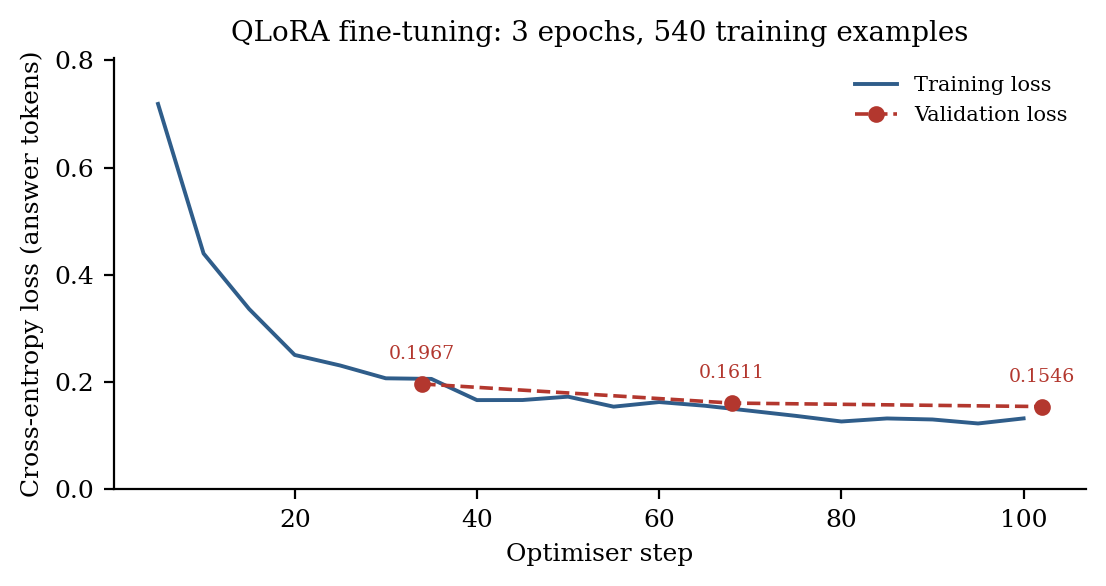
\includegraphics[width=0.72\textwidth]{fig_finetune_loss.png}
\caption{Fine-tuning loss. Validation loss decreases monotonically across all
three epochs, with no divergence between training and validation.}
\label{fig:ftloss}
\end{figure}

The monotone validation curve in Figure~\ref{fig:ftloss} indicates the model had
not begun to overfit within three epochs. The absolute loss values are low
because the task is highly structured---a fixed five-section format over a
constrained vocabulary---so this should be read as evidence of successful format
and style internalisation rather than of clinical competence, which is assessed
separately in Chapter~\ref{ch:results}.

\section{Safety Validator Implementation}
\label{sec:validator_method}

The validator is implemented in pure Python with no machine-learning
dependency, so that it runs identically in every deployment mode and can be
audited line by line. Detection is sentence-scoped and negation-aware: a
sentence is examined in isolation, and a candidate match is discarded if it is
governed by a negation or an explicit deferral to a clinician. This distinction
matters, because ``you should not stop or change any medicine without talking to
your doctor'' is safe guidance containing medication vocabulary, whereas
``stop taking your blood pressure medicine'' is a severe violation containing
similar vocabulary.

The severe family---diagnosis assertion, medication instruction, supplement
recommendation---triggers replacement with a safe template. The moderate
family---numeric nutrient targets, missing laboratory-confirmation reminder for
an at-risk result, and emergency indications---triggers in-place repair. A
structural check verifies that all five sections are present and, if not,
triggers a single regeneration before falling back.

Emergency handling deserves specific mention. The validator escalates on
measured vital signs (systolic $\geq$ 180 or diastolic $\geq$ 120 mmHg) and on
red-flag symptom vocabulary. In the current deployment the input schema exposes
no free-text symptom field, so the vitals path is the only one reachable from a
live request; the symptom vocabulary is nonetheless implemented, tested, and
exercised by the evaluation harness in Chapter~\ref{ch:results}, and is retained
for the schema extension discussed in Chapter~\ref{ch:conclusion}. This is
stated explicitly rather than left implicit, because the distinction between
``implemented and tested'' and ``reachable in production'' is exactly the kind of
gap that undermines a safety claim if glossed over.

\section{Citation Layer}
\label{sec:citations}

After validation, a deterministic citation layer attaches IEEE-style markers.
Each output section is mapped to the knowledge-base topics it may legitimately
draw upon---for example, \emph{Food habits} maps to \texttt{nutrition},
\texttt{diabetes} and \texttt{bp}---and is cited only to sources that were
actually retrieved for those topics in this request, refined by the grounding
identifiers the model itself reported. Numbering follows first-citation order
and the reference list de-duplicates by source document.

Because the mapping is computed from the retrieval record rather than parsed
from the generated text, a citation marker cannot point to a source the system
did not retrieve. Fabricated references---a well-documented failure mode of
generative models, and one a reviewing clinician would immediately catch---are
therefore structurally impossible rather than merely improbable.
